% Diapositiva 37

% David
%=============================================
% Punto 11: Gráfica Emin(z) — mejor error posible para cada profundidad.
%=============================================

\begin{frame}{Análisis de Profundidad: Gráfica $E_{\min}(z)$}

    \begin{columns}[T]

        \column{0.52\textwidth}

        \begin{block}{$E_{\min}(z)$: Valor mínimo del error por profundidad}
            \centering
            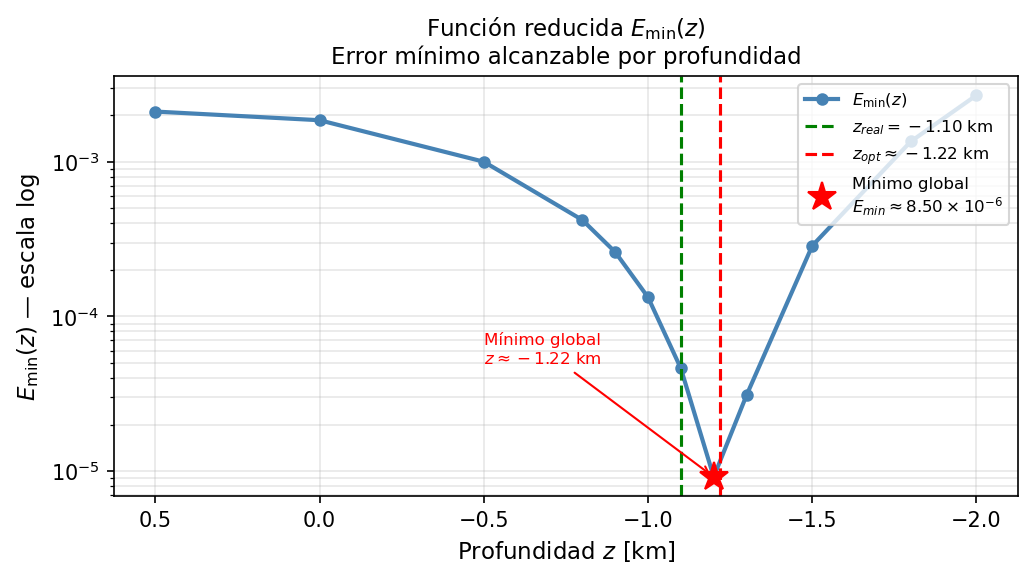
\includegraphics[width=0.95\textwidth]{Imagenes/emin_z.png}
        \end{block}

        \column{0.44\textwidth}

        \begin{block}{¿Qué representa esta gráfica?}
            \scriptsize
            \begin{itemize}
                \item Para cada $z$ se minimiza $E$ sobre $(x, y, A_0)$, obteniendo el \textbf{mejor ajuste posible} en ese plano.
                \vspace{0.15cm}
                \item La curva muestra \textbf{cómo varía la calidad del ajuste} según la profundidad.
                \vspace{0.15cm}
                \item El \textbf{mínimo global} $z_{opt} \approx -1.22$ km identifica la profundidad estimada del hipocentro.
            \end{itemize}
        \end{block}

        \vspace{0.2cm}

        \begin{exampleblock}{Interpretación Física}
            \scriptsize
            \begin{itemize}
                \item $z_{opt} \approx -1.22$ km con $E_{\min} \approx 8.50 \times 10^{-6}$
                \vspace{0.1cm}
                \item Diferencia con $z_{\text{real}} = -1.10$ km: solo \textbf{0.12 km}
                \vspace{0.1cm}
                \item La curvatura pronunciada indica \textbf{alta sensibilidad} del modelo a la profundidad.
            \end{itemize}
        \end{exampleblock}

    \end{columns}

    \vspace{0.15cm}
    \begin{center}
        \footnotesize
        \textbf{$E_{\min}(z)$ convierte el análisis 4D en una búsqueda unidimensional interpretable.}
    \end{center}

\end{frame}